\chapter{Redes neuronales}\label{Chapter7} 
% chktex-file 8
% chktex-file 12
% chktex-file 13
% chktex-file 44

Veremos redes neuronales poco profundas (no más de 2 capas ocultas). La idea básica es transformar un conjunto de variables capa a capa hasta llegar a un conjunto de variables fácilmente separables o ``regresables'' por la ultima capa. El resultado del pesado se pasa por una funcion de activacion no lineal. El peso $w_{ij}$ conecta la neurona j de la capa l con la neurona i de la capa l+1. No contamos el bias como neurona, asiq ue en el ejemplo que pone hay 3. El bias es un vector siempre, con dimension $\text{neuronas en esa capa} \times 1$. PAra el caso de la capa de entrada, la activacion es directametne la entrada. 

\section{Introducción}

Consideremos un problema de aprendizaje supervisado donde tenemos acceso a ejemplos de entrenamiento etiquetados $(x^{(i)}, y^{(i)})$. Las redes neuronales ofrecen una forma de definir una hipótesis compleja y no lineal $h_{W,b}(x)$, con parámetros $W, b$ que podemos ajustar a nuestros datos. \\

Para describir las redes neuronales, comenzaremos describiendo la red neuronal más simple posible, una que comprende una sola ``neurona''. Utilizaremos el diagrama \ref{fig:7.1} para denotar una sola neurona

\begin{figure}[H]
\centering
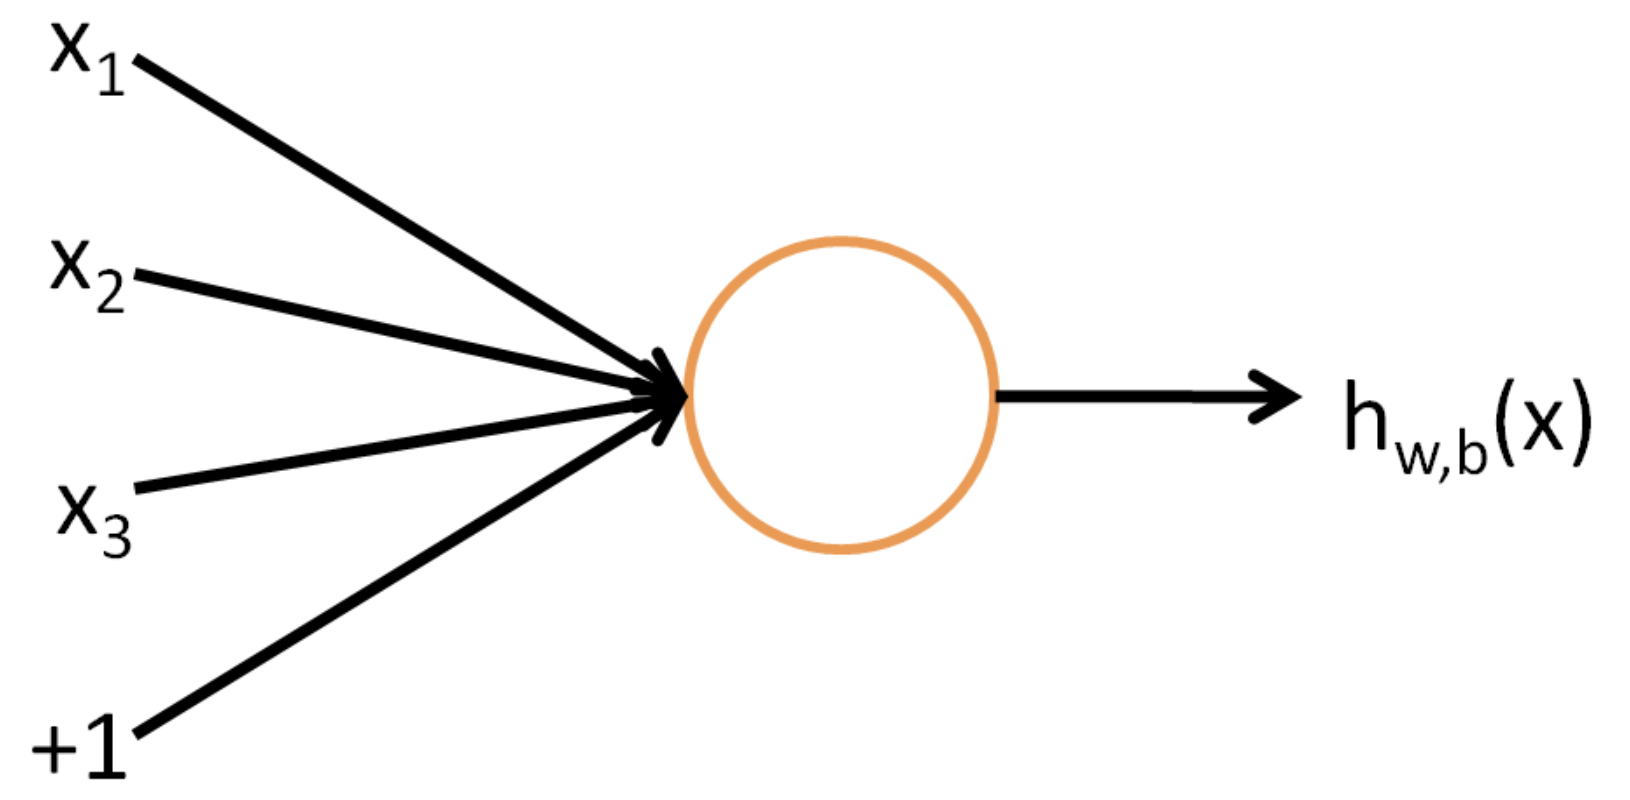
\includegraphics[width=0.4\textwidth]{fotos/40.png}
\caption{Diagrama de una neurona simple}
\label{fig:7.1}
\end{figure}

Esta ``neurona'' es una unidad computacional que toma como entrada $x_1, x_2, x_3$ (y un término de intercepto $+1$; este \textit{bias} no se cuenta como ``neurona''), y produce una salida 
\begin{equation}
h_{W,b}(x) = f(W^T x) = f\left(\sum_{i=1}^{3} W_i x_i + b\right)
\end{equation}

\noindent donde $f: \mathbb{R} \rightarrow \mathbb{R}$ se denomina función de activación. 

\subsection{Función de activación}

\subsubsection{Función sigmoide}

\noindent Aquí, elegiremos $f(\cdot)$ como la función sigmoide:
\begin{equation}
f(z) = \frac{1}{1 + e^{-z}}
\end{equation}

\noindent función acotada entre 0 y 1 también conocida como función logística estándar. Así, nuestra única neurona corresponde exactamente al mapeo de entrada-salida definido por la regresión logística. Una propiedad importante de esta función es que su derivada de puede escribir en términos de la misma función:
\begin{equation}
f'(z) = f(z)(1 - f(z))
\end{equation}

\begin{figure}[h]
\centering
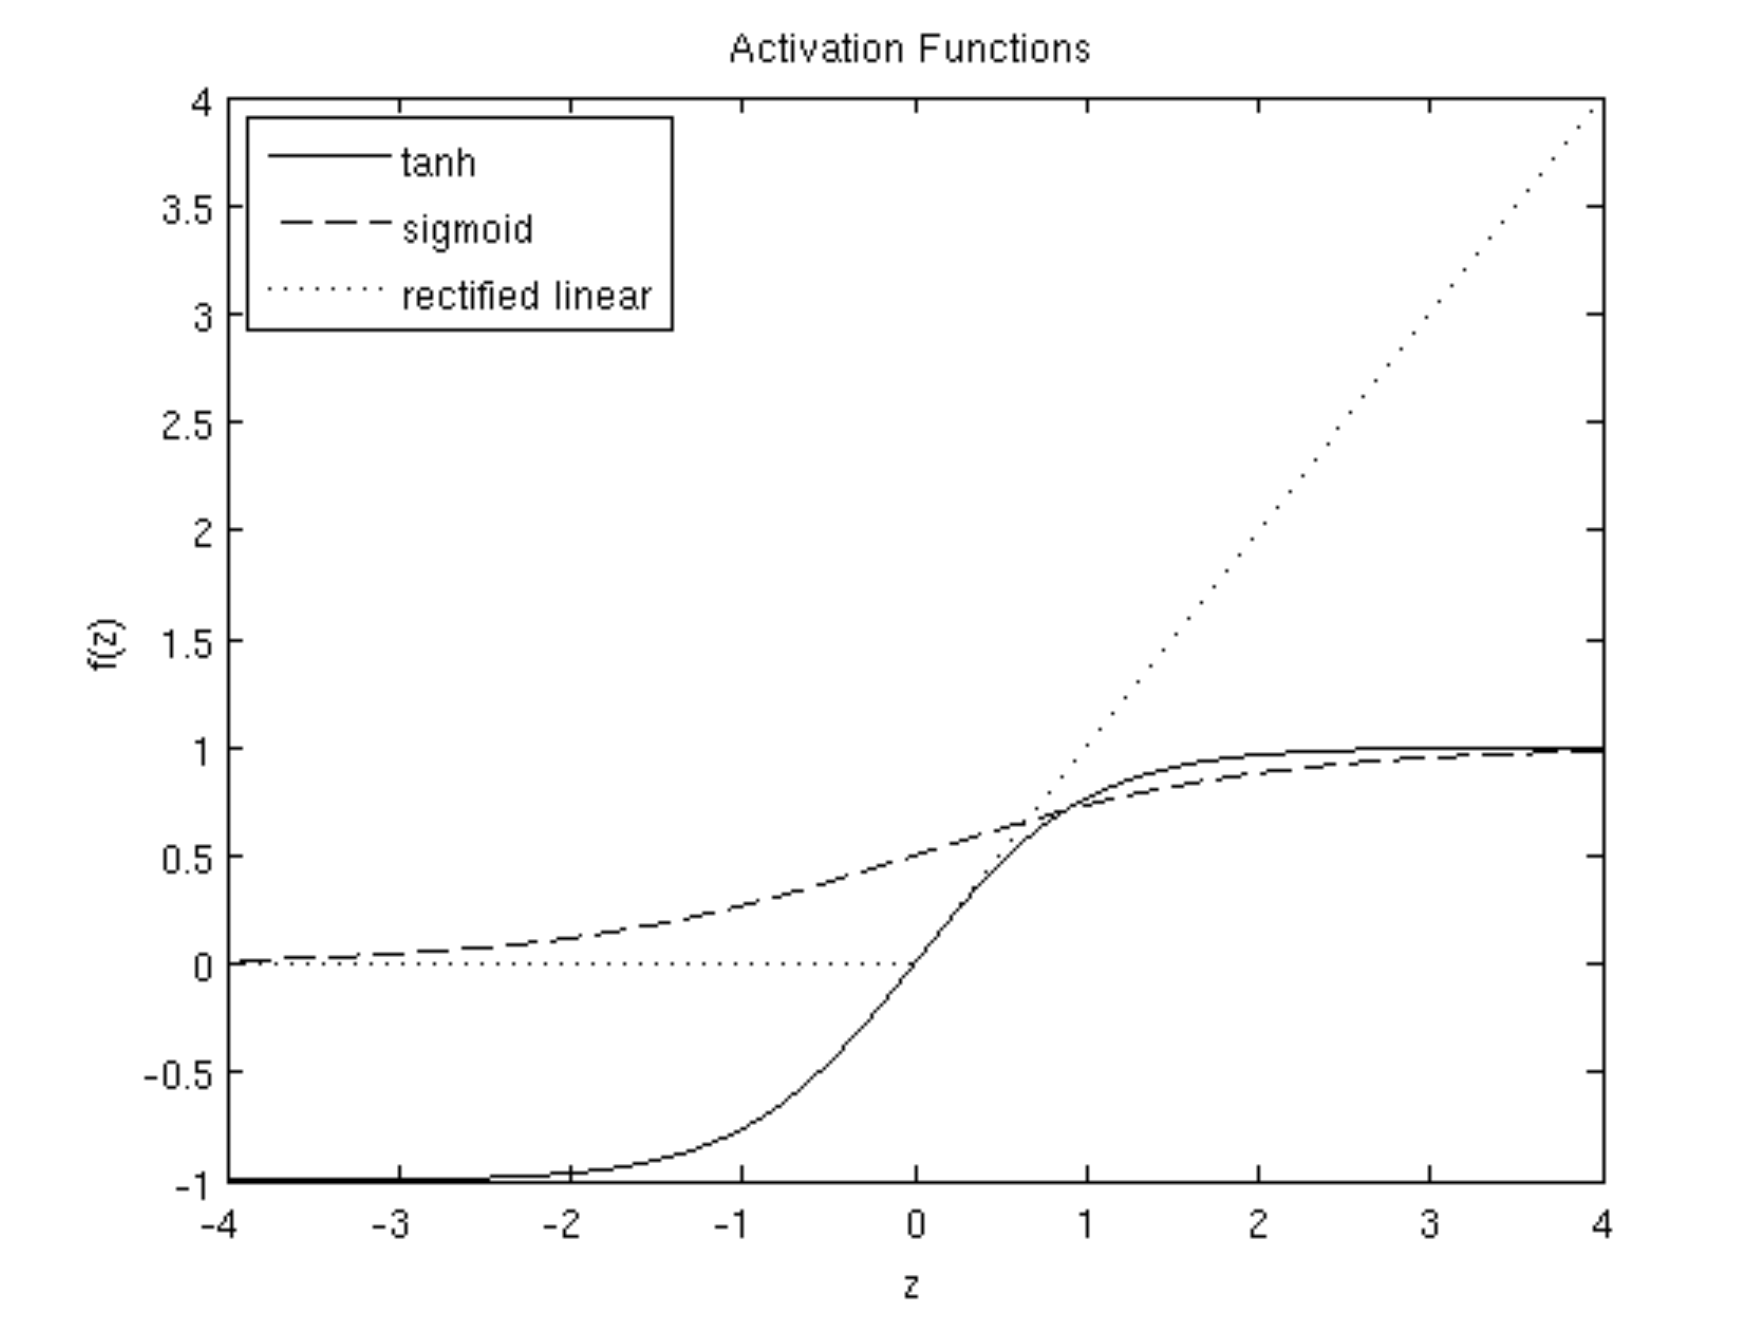
\includegraphics[width=0.6\textwidth]{fotos/41.png}
\caption{Funciones de activación: Sigmoide, tanh y ReLU}
\label{fig:7.2}
\end{figure}

\subsubsection{Tangente hiperbólica}

Aunque usaremos la función sigmoide, vale la pena notar que otra elección común para $f$ es la función tangente hiperbólica, o tanh:
\begin{equation}
f(z) = \tanh(z) = \frac{e^{z} - e^{-z}}{e^{z} + e^{-z}}
\end{equation}

La función $\tanh(z)$ es una versión reescalada de la sigmoide, y su rango de salida es $[-1, 1]$ en lugar de $[0,1]$. La derivada de esta función toma la forma $f'(z) = 1 - (f(z))^2$. 

\subsubsection{Función lineal rectificada ReLU}

Una función de activación diferente, la función lineal rectificada (ReLU), a menudo funciona mejor en la práctica para redes neuronales profundas. Esta función de activación es diferente de la sigmoide y la tanh porque no está acotada ni es continuamente diferenciable. La función de activación lineal rectificada se define como:
\begin{equation}
f(z) = \max(0, z)
\end{equation}

La función lineal rectificada es lineal por tramos y se satura exactamente en $0$ cuando la entrada $z$ es menor que $0$. Su derivada (gradiente) es 0 para $z<0$ y 1 para $z > 0$. El gradiente no está definido en $z = 0$, aunque esto no causa problemas en la práctica porque promediamos el gradiente sobre muchos ejemplos de entrenamiento durante la optimización.

\subsubsection{Funciones gaussianas de base radial}

El modelo de redes neuronales de funciones de base radial (RBF) es un modelo no lineal que utiliza funciones de base radial como funciones de activación. Las funciones de base radial son funciones que dependen solo de la distancia radial al origen, por lo que su valor es el mismo en todos los puntos que equidistan del origen. Sean matrices de covarianza cualesquiera, las funciones de base radial se definen como:
\begin{equation}
f_j(\mathbf{z}) = \exp\left\{-\frac{1}{2}(\mathbf{z} - \boldsymbol{\mu}_j)^T \boldsymbol{\Sigma}_j^{-1}(\mathbf{z} - \boldsymbol{\mu}_j)\right\}
\end{equation}

Como las matrices de covarianza son simétricas, se tiene que cada función de base radial tiene $d(d + 3)/2$ parámetros independientes ajustables, donde $d$ es la dimensión del espacio de entrada. \\


\section{Modelo de red neuronal}

Una red neuronal se construye conectando muchas ``neuronas'', de modo que la salida de una neurona puede ser la entrada de otra. Por ejemplo, la figura \ref{fig:7.3} muestra una pequeña red neuronal:

\begin{figure}[h]
\centering
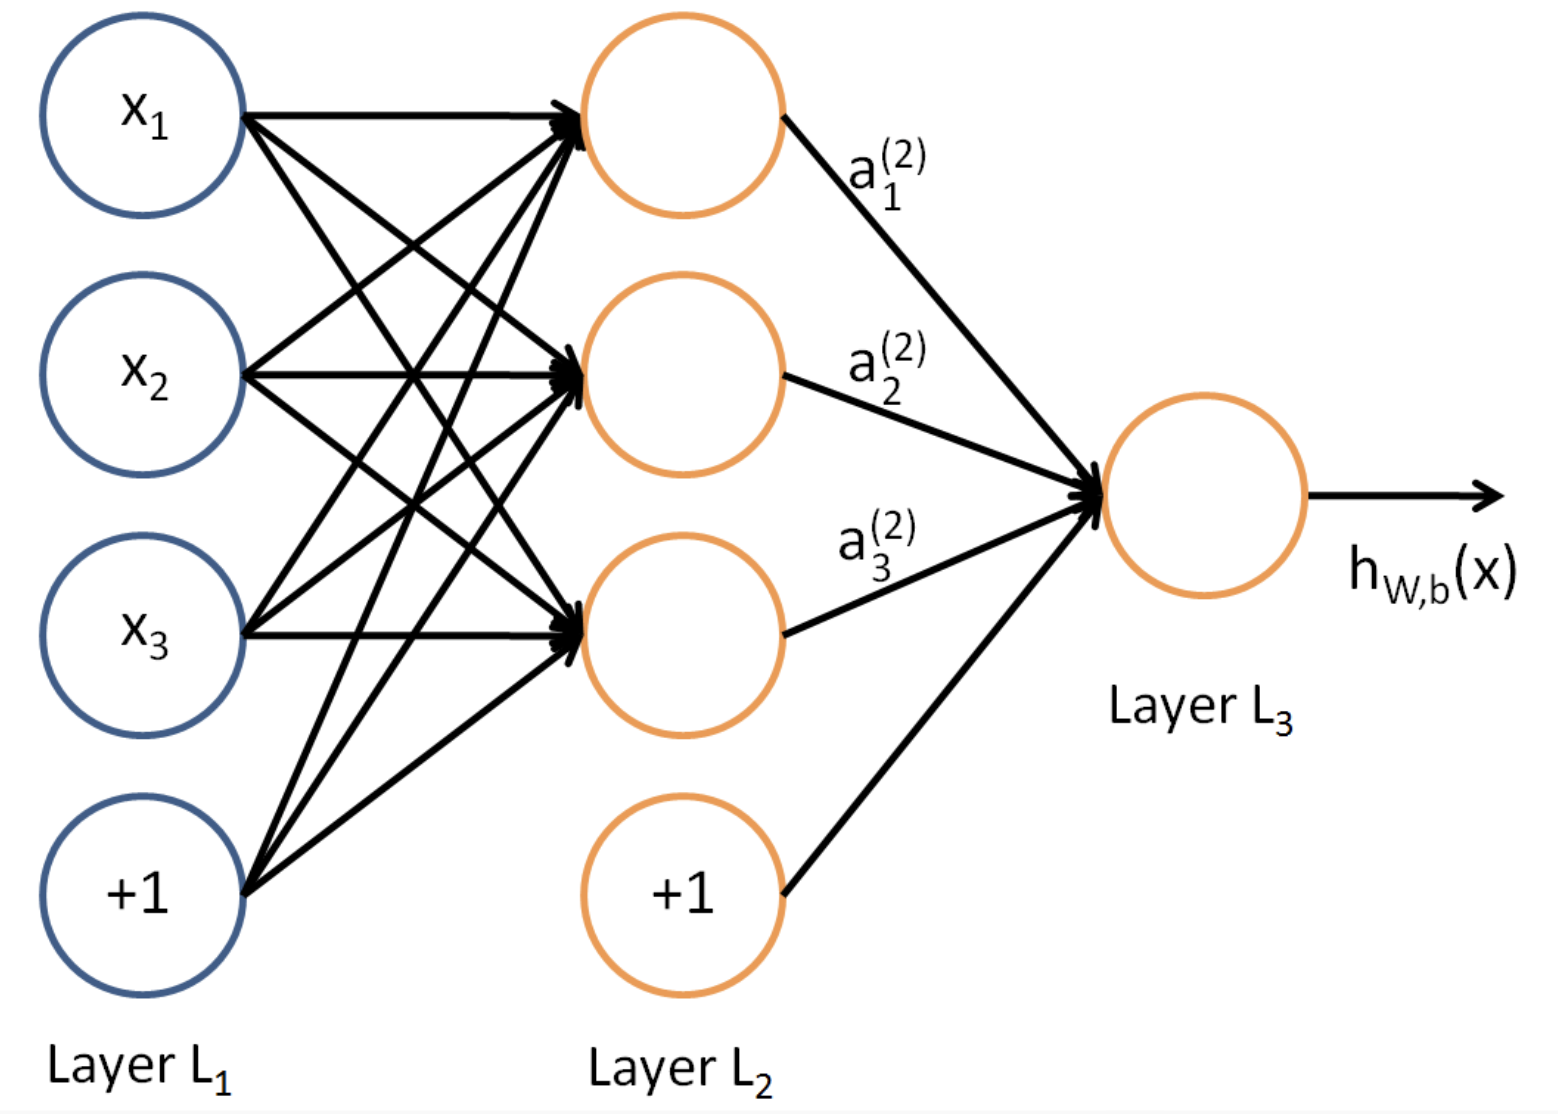
\includegraphics[width=0.5\textwidth]{fotos/42.png}
\caption{Ejemplo de una red neuronal pequeña}
\label{fig:7.3}
\end{figure}

En esta figura, hemos utilizado círculos para denotar también las entradas a la red. Los círculos etiquetados como ``+1'' se llaman unidades de sesgo y corresponden al término de intercepto. La capa más a la izquierda de la red se llama capa de entrada, y la capa más a la derecha la capa de salida (que, en este ejemplo, tiene solo una unidad). La capa intermedia de nodos se llama capa oculta, porque sus valores no se observan en el conjunto de entrenamiento. También decimos que nuestro ejemplo de red neuronal tiene 3 unidades de entrada (sin contar la unidad de sesgo), 3 unidades ocultas y 1 unidad de salida. \\

Denotaremos $n_l$ como el número de capas en nuestra red; por lo tanto, $n_l = 3$ en nuestro ejemplo. Etiquetamos la capa $l$ como $L_l$, por lo que la capa $L_1$ es la capa de entrada y la capa $L_{n_l}$ la capa de salida. \\

Nuestra red neuronal tiene parámetros $(W, b) = (W^{(1)}, b^{(1)}, W^{(2)}, b^{(2)})$, donde escribimos $W_{ij}^{(l)}$ para denotar el parámetro (o peso) asociado con la conexión entre la unidad $j$ en la capa $l$ y la unidad $i$ en la capa $l+1$ (nota el orden de los índices). Además, $b_i^{(l)}$ es el sesgo asociado con la unidad $i$ en la capa $l+1$. Así, en nuestro ejemplo, tenemos $W^{(1)} \in \mathbb{R}^{3 \times 3}$ y $W^{(2)} \in \mathbb{R}^{1 \times 3}$. Note que las unidades de sesgo no tienen entradas ni conexiones entrantes, ya que siempre sacan el valor $+1$; en nuestro ejemplo $b^{(1)} \in \mathbb{R}^{3 \times 1}$ y $b^{(2)} \in \mathbb{R}^{1 \times 1}$. También denotamos $s_l$ como el número de nodos en la capa $l$ (sin contar la unidad de sesgo). \\

Escribiremos $a^{(l)}_i$ para denotar la activación (es decir, el valor de salida) de la unidad $i$ en la capa $l$. Para $l = 1$, también usamos $a^{(1)}_i = x_i$ para denotar la $i$-ésima entrada. En lo sucesivo, también denotamos $z^{(l)}_i$ como la suma ponderada total de entradas a la unidad $i$ en la capa $l$, incluyendo el término de sesgo,  
\begin{equation}
z_i^{(l+1)} = \sum_{j=1}^{s_l} W_{ij}^{(l)} a_j^{(l)} + b_i^{(l)}
\end{equation}

\noindent de modo que $a^{(l)}_i = f(z^{(l)}_i)$. Dado un conjunto fijo de parámetros $W, b$, nuestra red neuronal define una hipótesis $h_{W,b}(x)$ que produce un número real. Específicamente, el cómputo que esta red neuronal representa se da por:

\begin{align}
a_1^{(2)} &= f\left(W_{11}^{(1)} x_1 + W_{12}^{(1)} x_2 + W_{13}^{(1)} x_3 + b_1^{(1)}\right) \\
a_2^{(2)} &= f\left(W_{21}^{(1)} x_1 + W_{22}^{(1)} x_2 + W_{23}^{(1)} x_3 + b_2^{(1)}\right) \\
a_1^{(2)} &= f\left(W_{31}^{(1)} x_1 + W_{32}^{(1)} x_2 + W_{33}^{(1)} x_3 + b_3^{(1)}\right) \\
h_{W, b}(x) &= a_1^{(3)} = f\left(W_{11}^{(2)} a_1^{(2)} + W_{12}^{(2)}a_2^{(2)} + W_{13}^{(2)} a_3^{(2)} + b_1^{(2)}\right)
\end{align}

Nótese que esto se presta fácilmente a una notación más compacta. Específicamente, si extendemos la función de activación $f(\cdot)$ para que se aplique a vectores de manera elemento a elemento (es decir, $f([z_1, z_2, z_3]) = [f(z_1), f(z_2), f(z_3)]$), entonces podemos escribir las ecuaciones anteriores de manera más compacta como:
\begin{align}
z^{(2)} &= W^{(1)} x + b^{(1)} \\
a^{(2)} &= f(z^{(2)}) \\
z^{(3)} &= W^{(2)} a^{(2)} + b^{(2)} \\
h_{W,b}(x) &= a^{(3)} = f(z^{(3)})
\end{align}

Llamamos a este paso propagación hacia adelante (\textit{forward propagation}). Más generalmente, recordando que también usamos $a^{(1)} = x$ para denotar los valores de la capa de entrada, dadas las activaciones $a^{(l)}$ de la capa $l$, podemos calcular las activaciones $a^{(l+1)}$ de la capa $l+1$ como:
\begin{align}
z^{(l+1)} &= W^{(l)} a^{(l)} + b^{(l)} \\
a^{(l+1)} &= f(z^{(l+1)})
\end{align}

Al organizar nuestros parámetros en matrices y utilizando operaciones de álgebra lineal vectorial, podemos aprovechar rutinas rápidas de álgebra lineal para realizar cálculos en nuestra red de manera eficiente. \\

\section{Arquitecturas}

Hasta ahora, nos hemos centrado en un ejemplo de red neuronal, pero también se pueden construir redes neuronales con otras arquitecturas (es decir, patrones de conectividad entre neuronas), incluyendo aquellas con múltiples capas ocultas. Las capas pueden estar conectadas densamente, como en nuestro ejemplo, o pueden tener conexiones más dispersas (locales, \textit{locally connected}), en cuyo caso se pueden compartir los pesos. \\

La elección más común es una red de $n_l$ capas donde la capa $1$ es la capa de entrada, la capa $n_l$ es la capa de salida, y cada capa $l$ está densamente conectada a la capa $l+1$. En este contexto, para computar la salida de la red, podemos calcular sucesivamente todas las activaciones en la capa $L_2$, luego en la capa $L_3$, y así sucesivamente, hasta la capa $L_{n_l}$, utilizando las ecuaciones anteriores que describen el paso de propagación hacia adelante. Este es un ejemplo de una red neuronal \textit{feedforward}, ya que el grafo de conectividad no tiene bucles ni ciclos dirigidos. \\

Las redes neuronales también pueden tener múltiples unidades de salida. Por ejemplo, en la figura \ref{fig:7.4} hay una red con dos capas ocultas $L_2$ y $L_3$ y dos unidades de salida en la capa $L_4$.

\begin{figure}[h]
\centering
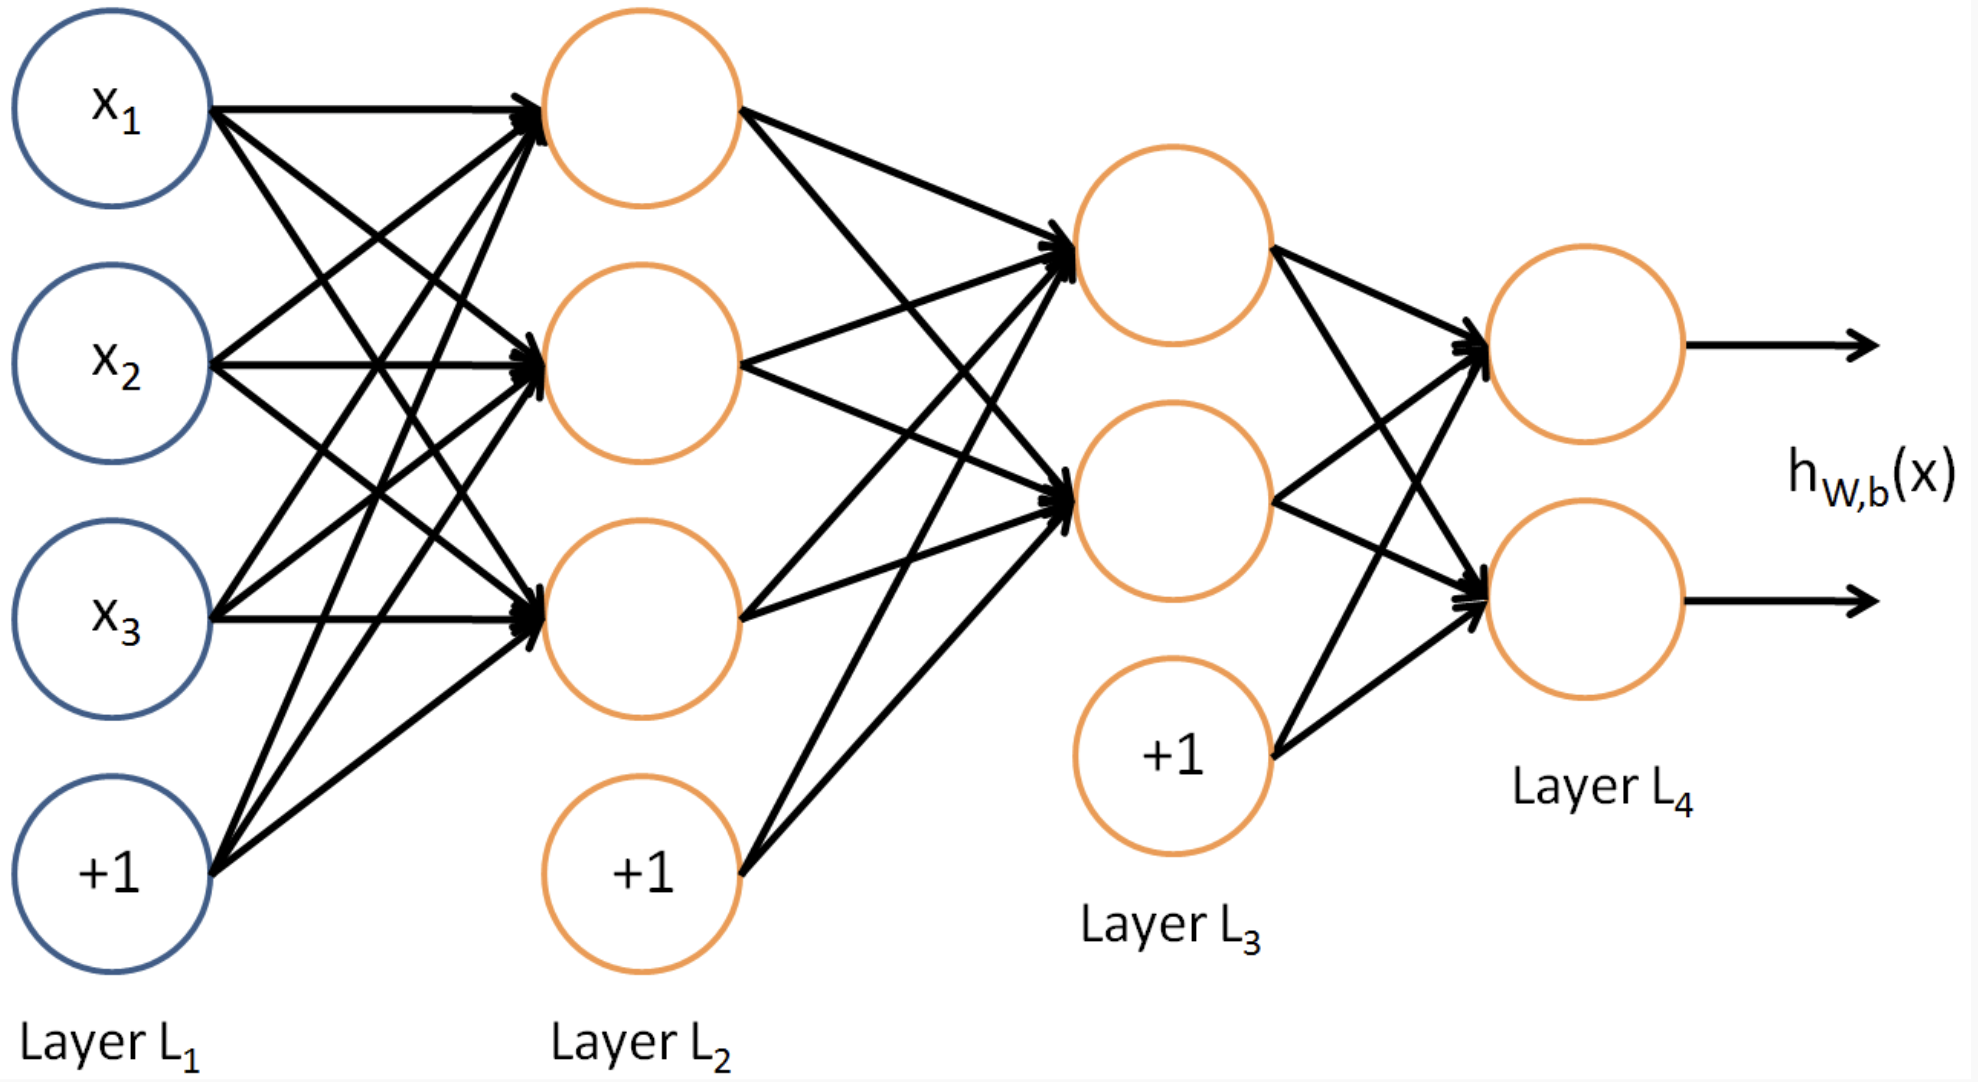
\includegraphics[width=0.6\textwidth]{fotos/43.png}
\caption{Red neuronal con múltiples capas ocultas y múltiples unidades de salida.}
\label{fig:7.4}
\end{figure}

Para entrenar esta red, necesitaríamos ejemplos de entrenamiento $(x^{(i)}, y^{(i)})$ donde $y^{(i)} \in \mathbb{R}^2$. Este tipo de red es útil si hay múltiples salidas que te interesa predecir. Por ejemplo, en una aplicación de diagnóstico médico, el vector $x$ podría proporcionar las características de entrada de un paciente, y las diferentes salidas $y_i$ podrían indicar la presencia o ausencia de diferentes enfermedades. \\

Dependiendo del tipo de problema a afrontar, se toman ciertas consideraciones generales: 
\begin{itemize}
\item Regresión.
\begin{itemize}
\item Una salida por cada variable de salida.
\item La función de salida es generalmente la función identidad.
\item Estandarización de los datos (entradas y salidas), ya que el rango depende de la función de activación.
\end{itemize}
\item Clasificación. 
\begin{itemize}
\item Para clasificación binaria, se utiliza una única unidad de salida y la sigmoide como función de salida.
\item Para una clasificación de $K$ clases, se utilizan $K$ unidades de salida: \textit{encoding} $[1 \; 0 \; 0 \; 0]^T$, $[0 \; 1 \; 0 \; 0]^T$, $[0 \; 0 \; 1 \; 0]^T$, $[0 \; 0 \; 0 \; 1]^T$.
\item La función de salida es generalmente la función \textit{softmax}.
\begin{equation}
f(z_i^{(l)}) = \frac{\exp(z_i^{(l)})}{\sum_{j = 1}^K \exp(z_j^{(l)})}
\end{equation}
\begin{example}
Salida de la función \textit{softmax} para un caso de clasificación de 3 clases: bicicleta, coche y camión.
\begin{table}[H]
\centering
\begin{tabular}{ccccc}
\hline \hline
 & $z_i$ & $\exp(z_i)$ & $f(z_i)$ & Prob. correctas \\ \hline \hline
Bicicleta & $-0.2$ & $0.8$ & $0.2$ (2\%) & $0.00$ \\
Coche & $3.6$ & $36.6$ & $0.75$ (75\%) & $1.00$ \\
Camión & $2.4$ & $11.0$ & $0.23$ (23\%) & $0.00$ \\ \hline 
\end{tabular}
\end{table}
\end{example}
\end{itemize}
\end{itemize}

\section{Funciones de coste o error}

Sea un conjunto de entrenamiento $\{(x^{(1)}, y^{(1)}), \ldots, (x^{(m)}, y^{(m)})\}$. 

\subsection{Logartimo negativo de la verosimilitud}

Intuitivamente, queremos maximizar la probabilidad de verosimilitud sobre los datos de entrenamiento; esto es, cada punto de datos se asume que se genera a partir de la misma distribución de probabilidad
\begin{equation}
\mathcal{P} = \prod_{i = 1}^m p(x_i, y_i) = \prod_{i = 1}^m p(y_i \mid x_i) p(x_i)
\end{equation}

Sin embargo, el producto de probabilidades en poco estable numéricamente (se obtienen valores muy pequeños), por lo que se suele usar el logaritmo negativo de la verosimilitud como función de coste (a minimizar):
\begin{equation}
J = -\log \mathcal{P} = -\sum_{i = 1}^m \log p(y_i \mid x_i) - \log \sum_{i = 1}^m p(x_i) = -\sum_{i = 1}^m \log p(y_i \mid x_i)
\end{equation}

\subsection{Suma del error cuadrático}

\noindent Si se asume que la distribución de los datos es gaussiana,
\begin{equation}
p(y \mid x) = \prod_{i = 1}^m \frac{1}{(2\pi \sigma^2)^{1/2}} \exp\left(-\frac{(h(x_i) - y_i)^2}{2\sigma^2}\right)
\end{equation} 

\noindent se puede usar la suma del error cuadrático como función de coste:
\begin{equation}
J = \frac{1}{2} \sum_{i = 1}^m (h(x_i) - y_i)^2
\end{equation}

\subsection{Entropía cruzada}

\subsubsection{Entropía cruzada binaria}

\noindent Para problemas de clasificación binaria, se puede usar la entropía binaria cruzada como función de coste:
\begin{itemize}
\item Para una sola unidad de salida: $p(\mathcal{C}_1 \mid x_i) = h(x_i)$ y $p(\mathcal{C}_2 \mid x_i) = 1 - h(x_i)$
\item La función de salida es la sigmoide, por lo que se interpreta como una probabilidad.
\end{itemize}

\noindent En caso de tener más de una unidad de salida,
\begin{equation}
p(y_i \mid x_i) = (h(x_i))^y_i (1 - h(x_i))^{1 - y_i}
\end{equation}

\noindent y la función de coste es
\begin{equation}
J = -\sum_{i = 1}^m \left(y_i \log h(x_i) + (1 - y_i) \log (1 - h(x_i))\right)
\end{equation}

Esta función de error es mínima cuando las predicciones del modelo coinciden con las etiquetas reales, esto es $h(x_i) = y_i$. La derivada de esta función respecto a la salida del modelo $h(x_i)$ es
\begin{equation}
\frac{\partial J}{\partial h(x_i)} = \frac{h(x_i) - y_i}{h(x_i)(1 - h(x_i))}
\end{equation}

\subsubsection{Entropía cruzada}

\noindent Para problemas de clasificación multiclase ($K$ clases), con clases mutuamente excluyentes, se tiene que 
\begin{align}
p (\mathcal{C}_k \mid x_i) &= h^k(x_i) \\
p (y_i \mid x_i) &= \prod_{k = 1}^K (h^k(x_i))^{y_i^k}
\end{align}

donde el superíndice $k$ simplemente indica la clase $k$-ésima. La función de coste asociada es 
\begin{equation}
J = -\sum_{i = 1}^m \sum_{k = 1}^K y_i^k \log h^k(x_i)
\end{equation}

En el caso de tener $K$ clases mutuamente no excluyentes, se asume independencia en las categorías, esto es
\begin{equation}
p (y_i \mid x_i) = \prod_{k = 1}^K (h^k(x_i))^{y_i^k} (1 - h^k(x_i))^{1 - y_i^k}
\end{equation}

\noindent y la función de error se escribe como 
\begin{equation}
J = -\sum_{i = 1}^m \sum_{k = 1}^K \left(y_i^k \log h^k(x_i) + (1 - y_i^k) \log (1 - h^k(x_i))\right)
\end{equation}

Ambas funciones de coste tienen un mínimo de error en $h^k(x_i) = y_i^k$. Los valores de salida pasan por una \textit{softmax}, por lo que se interpretan como probabilidades.

\begin{example}
Sean tres clases mutuamente excluyentes: bicicleta, coche y camión. Suponemos que la salida de la función \textit{softmax} es 
\begin{table}[H]
\centering
\begin{tabular}{cc}
\hline \hline
Clase & \textit{softmax} \\ \hline \hline
Bicicleta ($k = 1$) & 0.02 \\
Coche ($k = 2$) & 0.75 \\
Camión ($k = 3$) & 0.23 \\ \hline
\end{tabular}
\end{table}

\noindent La función de coste, al ser clases mutuamente excluyentes, es
\begin{equation}
J = -\sum_{i = 1}^m \sum_{k = 1}^K y_i^k \log h^k(x_i)
\end{equation}

\noindent Así, $J = - (0.0 - 0.29 - 0.0) = 0.29$ ya que  
\begin{itemize}
\item $k = 1$: $0 \cdot \log (0.02) = 0.0$
\item $k = 2$: $1 \cdot \log (0.75) = -0.29$
\item $k = 3$: $0 \cdot \log (0.23) = 0.0$
\end{itemize}

Dependiendo de las probabilidades de salida, se obtiene un valor de error distinto que nos indica cuán bien está clasificando el modelo. Supongamos varios casos:
\begin{table}[H]
\centering
\begin{tabular}{cccl}
\hline \hline
Clase real & \textit{softmax}(h) & $J$ &  \\ \hline \hline
Coche & $\{0.02, \textcolor{green}{0.75}, 0.23\}$ & $0.29$ & Buen clasificador \\
Coche & $\{0.00, \textcolor{green}{1.00}, 0.00\}$ & $0.00$ & Clasificador perfecto \\
Camión & $\{0.00, \textcolor{red}{0.75}, 0.25\}$ & $1.39$ & Mal clasificador \\
Camión & $\{0.00, \textcolor{red}{1.00}, 0.00\}$ & $\gg$ & El peor clasificador posible \\
\end{tabular}
\end{table}
\end{example}

\section{Ajuste de la red}

\subsection{Problema de optimización}

Sea un conjunto de entrenamiento $\{(x^{(1)}, y^{(1)}), \ldots, (x^{(m)}, y^{(m)})\}$. La función de coste global tendrá la forma 
\begin{equation}
J(W, b) = \frac{1}{m} \sum_{e = 1}^m J(W, b; x^{(e)}, y^{(e)}) + \lambda R(W)
\end{equation}

Si aplicamos una regularización $L_2$, la función de coste global se escribe como
\begin{align}
J(W, b) &= \frac{1}{m} \sum_{e = 1}^m J(W, b; x^{(e)}, y^{(e)}) + \frac{\lambda}{2} \sum_{l = 1}^{n_l - 1} \sum_{i = 1}^{s_l} \sum_{j = 1}^{s_{l+1}} (W_{ij}^{(l)})^2 \notag \\
&= \frac{1}{2m} \sum_{e = 1}^m ||h_{W, b}(x^{(e)}) - y^{(e)}||^2 + \frac{\lambda}{2} \sum_{l = 1}^{n_l - 1} \sum_{i = 1}^{s_l} \sum_{j = 1}^{s_{l+1}} (W_{ji}^{(l)})^2
\end{align} 

\noindent El primer término es un término de error promedio de suma de cuadrados. El segundo término es de regularización (también llamado término de decaimiento del peso) que tiende a disminuir la magnitud de los pesos y ayuda a prevenir el sobreajuste. \\

Por lo general, el decaimiento del peso no se aplica a los términos de sesgo $b^{(l)}_i$, como se refleja en la definición de $J(W,b)$. Aplicar decaimiento del peso a las unidades de sesgo generalmente solo hace una pequeña diferencia en la red final. \\

El parámetro de decaimiento del peso $\lambda$ controla la importancia relativa de los dos términos. Nota también la notación ligeramente sobrecargada: $J(W,b;x,y)$ es el costo de error cuadrático con respecto a un solo ejemplo; $J(W,b)$ es la función de costo global, que incluye el término de decaimiento del peso. \\

Esta función de costo se utiliza a menudo tanto para problemas de clasificación como de regresión. Para clasificación, dejamos que $y=0$ o $1$ representen las dos etiquetas de clase (recuerda que la función de activación sigmoide produce valores en [0,1]. Para el caso de una función de activación tanh, en su lugar usaríamos -1 y +1 para denotar las etiquetas). Para problemas de regresión, primero escalamos nuestras salidas para asegurarnos de que estén en el rango [0,1] (o si estuviéramos usando una función de activación tanh, entonces el rango [-1,1]). \\

El objetivo es encontrar el $W$ que minimice $J(W,b)$. Para entrenar nuestra red neuronal, inicializaremos cada parámetro $W^{(l)}_{ij}$ y cada $b^{(l)}_i$ a un valor aleatorio pequeño cerca de cero (digamos según una distribución Normal(0, $\epsilon^2$) para algún pequeño $\epsilon$, por ejemplo $0.01$), y luego aplicaremos un algoritmo de optimización como el descenso de gradiente por lotes (\textit{batches}). Dado que $J(W,b)$ es una función no convexa, el descenso de gradiente es susceptible a óptimos locales. Sin embargo, el descenso de gradiente generalmente funciona bastante bien. \\

Es importante inicializar los parámetros aleatoriamente, en lugar de todos en 0. Si todos los parámetros comienzan con valores idénticos, entonces todas las unidades de la capa oculta terminarán aprendiendo la misma función de la entrada (más formalmente, $W^{(1)}_{ij}$ serán iguales para todos los valores de $i$, de modo que $a^{(2)}_1 = a^{(2)}_2 = a^{(2)}_3 = \dots$ para cualquier entrada $x$). La inicialización aleatoria sirve para romper la simetría. \\

\noindent El gradiente analítico es un método exacto y rápido. Una iteración del descenso de gradiente actualiza los parámetros $W,b$ como sigue
\begin{align}
W^{(l)}_{ij} &:= W^{(l)}_{ij} - \alpha \frac{\partial J (W, b)}{\partial W^{(l)}_{ij}} \\
b^{(l)}_i &:= b^{(l)}_i - \alpha \frac{\partial J (W, b)}{\partial b^{(l)}_i}
\end{align}

donde $\alpha$ es la tasa de aprendizaje (en la figura \ref{fig:7.5} se mustra el efecto del valor de $\alpha$ sobre la pérdida o error). El paso clave es calcular las derivadas parciales anteriores. Ahora describiremos el algoritmo de retropropagación (\textit{backpropagation}), que proporciona una manera eficiente de calcular estas derivadas parciales. \\

\begin{figure}[h]
\centering
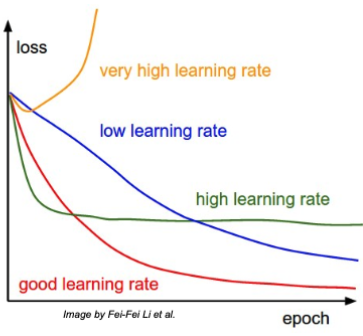
\includegraphics[width=0.35\textwidth]{fotos/44.png}
\caption{Curva de entrenamiento de una red para varios valores (cualitativos) de $\alpha$.}
\label{fig:7.5}
\end{figure}

\subsection{Retropropagación}

Primero describiremos cómo la retropropagación puede utilizarse para calcular $\partial_{W^{(l)}_{ij}}J$ y $\partial_{b^{(l)}_{i}}J$, las derivadas parciales de la función de costo $J(W,b;x,y)$ definida con respecto a un solo ejemplo $(x, y)$. Una vez que podamos calcular estas, vemos que la derivada de la función de costo global $J(W,b)$ puede calcularse como:
\begin{align}
\frac{\partial J(W,b)}{\partial W^{(l)}_{ij}} &= \frac{1}{m} \sum_{e = 1}^m \frac{\partial J(W,b;x^{(e)},y^{(e)})}{\partial W^{(l)}_{ij}} + \lambda W^{(l)}_{ij} \\
\frac{\partial J(W,b)}{\partial b^{(l)}_i} &= \frac{1}{m} \sum_{e = 1}^m \frac{\partial J(W,b;x^{(e)},y^{(e)})}{\partial b^{(l)}_i}
\end{align}

Las dos líneas anteriores difieren ligeramente porque el decaimiento de peso se aplica a $W$ pero no a $b$. \\

La intuición detrás del algoritmo de retropropagación es la siguiente. Dado un ejemplo de entrenamiento $(x, y)$, primero realizaremos una ``pasada hacia adelante'' para calcular todas las activaciones a lo largo de la red, incluyendo el valor de salida de la hipótesis $h_{W,b}(x)$. Luego, para cada nodo $i$ en la capa $l$, nos gustaría calcular un ``término de error'' $\delta^{(l)}_i$ que mida cuánto de responsable fue ese nodo de cualquier error en nuestra salida. Para un nodo de salida, podemos medir directamente la diferencia entre la activación de la red y el valor objetivo real, y usar eso para definir $\delta^{(n_l)}_i$ (donde la capa $n_l$ es la capa de salida). Para las unidades, calcularemos $\delta^{(l)}_i$ basadonos en un promedio ponderado de los términos de error de los nodos que utilizan $a^{(l)}_i$ como entrada. En detalle, aquí está el algoritmo de retropropagación:
\begin{itemize}
\item Realizamos un ``barrido hacia delante', calculando las activaciones para cada capa hasta la capa de salida: $L_2, L_3, \dots, L_{n_l}$.
\item Para cada unidad de salida $i$ en la capa de salida $n_l$, fijamos
\begin{equation}
\delta^{(n_l)}_i = \frac{\partial}{\partial z^{(n_l)}_i} \frac{1}{2} ||h_{W,b}(x) - y||^2 = )a^{(n_l)}_i - y_i) \cdot f'(z^{(n_l)}_i)
\end{equation}
Esto es así si la función de error es la suma de los cuadrados, sino, hay que reemplazar con la función adecuada. Concretamente, 
\begin{equation}
\delta^{(n_l)}_i = \frac{\partial J(W, b; x, y)}{\partial z^{(n_l)}_i} = \sum_{j = 1}^{s_l + 1} \frac{\partial J(W, b; x, y)}{\partial z_j^{(l+1)}} \frac{\partial z_j^{(l+1)}}{\partial z_i^{(l)}} = \sum_{j = 1}^{s_l + 1} \delta^{(l + 1)}_j \frac{\partial z_j^{(l+1)}}{\partial z_i^{(l)}}
\end{equation}
\item Para $l = n_l - 1, n_l - 2, \dots, 2$,
\begin{itemize}
\item Para cada nodo $i$ en la capa $l$, fijamos
\begin{equation}
\delta^{(l)}_i = \left(\sum_{j = 1}^{s_{l+1}} W_{ji}^{(l)} \delta^{(l+1)}_j\right) f'(z^{(l)}_i)
\end{equation}
Concretamente, dado $a_i^{(l)} = f(z_i^{(l)})$,
\begin{equation}
z_i^{(l+1)} = \sum_{j = 1}^{s_l} W_{ij}^{(l)} a_j^{(l)} + b_i^{(l)} = \sum_{j = 1}^{s_l} W_{ij}^{(l)} f(z_j^{(l)}) + b_i^{(l)}
\end{equation}
Entonces,
\begin{align}
\frac{\partial z_j^{(l+1)}}{\partial z_i^{(l)}} &= W_{ji}^{(l)} f'(z_i^{(l)}) \\
\delta_i^{(l)} &= \sum_{j = 1}^{s_l + 1} \delta_j^{(l+1)} \frac{\partial z_j^{(l+1)}}{\partial z_i^{(l)}} = \left(\sum_{j = 1}^{s_{l+1}} W_{ji}^{(l)} \delta_j^{(l+1)}\right) f'(z_i^{(l)})
\end{align}
\end{itemize}
\item Calcular las derivadas parciales deseadas, que vienen dadas por 
\begin{align}
\frac{\partial J(W,b;x,y)}{\partial W^{(l)}_{ij}} &= \frac{\partial z_i^{(l+1)}}{\partial W_{ij}^{(l)}}\frac{\partial J(W, b; x, y)}{\partial z_i^{(l + 1)}} = a^{(l)}_i \delta^{(l+1)}_j \\
\frac{\partial J(W,b;x,y)}{\partial b^{(l)}_i} &= \delta^{(l+1)}_i
\end{align}
\end{itemize}

Finalmente, también podemos reescribir el algoritmo utilizando notación matricial. Usaremos ``$\circ$'' para denotar el operador de producto elemento a elemento (producto de Hadamard), de modo que si $a = b \circ c$, entonces $a_i = b_i c_i$. Similar a cómo extendimos la definición de $f(\cdot)$ para aplicarla elemento a elemento a vectores, también hacemos lo mismo para $f'(\cdot)$ (de modo que $f'([z_1,z_2,z_3]) = [f'(z_1), f'(z_2), f'(z_3)]$). El algoritmo se reescribe como sigue:
\begin{itemize}
\item Realizamos un ``barrido hacia delante', calculando las activaciones para cada capa hasta la capa de salida: $L_2, L_3, \dots, L_{n_l}$. Esto se hace con las ecuaciones ya vistas en la propagación hacia delante.
\item Para la capa de salida $n_l$, fijamos
\begin{equation}
\delta^{(n_l)} = (a^{(n_l)} - y) \circ f'(z^{(n_l)})
\end{equation}
\item Para $l = n_l - 1, n_l - 2, \dots, 2$, fijamos
\begin{equation}
\delta^{(l)} = ((W^{(l)})^T \delta^{(l+1)}) \circ f'(z^{(l)})
\end{equation}
\item Calculamos las derivadas parciales:
\begin{align}
\nabla_{W^{(l)}} J(W, b; x, y) &= \delta^{(l+1)} (a^{(l)})^T \\
\nabla_{b^{(l)}} J(W, b; x, y) &= \delta^{(l+1)}
\end{align}
\end{itemize}

En los pasos 2 y 3 anteriores, necesitamos calcular $f'(z^{(l)}_i)$ para cada valor de $i$. Asumiendo que $f(z)$ es la función de activación sigmoide, ya tendríamos almacenado $a^{(l)}_i$ desde la pasada hacia adelante a través de la red. Así, utilizando la expresión que desarrollamos anteriormente para $f'(z)$, podemos calcular esto como $f'(z^{(l)}_i) = a^{(l)}_i(1 - a^{(l)}_i)$.

\subsection{Descenso de gradiente}

Finalmente, estamos listos para describir el algoritmo completo de descenso de gradiente. En el pseudo-código a continuación, $\Delta W^{(l)}$ es una matriz (de la misma dimensión que $W^{(l)}$), y $\Delta b^{(l)}$ es un vector (de la misma dimensión que $b^{(l)}$). Nota que en esta notación, ``$\Delta W^{(l)}$'' es una matriz, no es ``$\Delta$ por $W^{(l)}$''. Implementamos una iteración del descenso de gradiente por lotes de la siguiente manera:
\begin{itemize}
\item Fijamos $\Delta W^{(l)} := 0$ y $\Delta v^{(l)} := 0$ $\forall l$ (matrices/vectores de ceros).
\item Desde $i = 1$ hasta $m$:
\begin{itemize}
\item Usar retropropagación para calcular $\nabla_{W^{(l)}} J(W, b; x, y)$ y $\nabla_{b^{(l)}} J(W, b; x, y)$.
\item Fijar $\Delta W^{(l)} := \Delta W^{(l)} + \nabla_{W^{(l)}} J(W, b; x, y)$. 
\item Fijar $\Delta b^{(l)} := \Delta b^{(l)} + \nabla_{b^{(l)}} J(W, b; x, y)$.
\end{itemize}
\item Actualizar los parámetros:
\begin{align}
W^{(l)} &:= W^{(l)} - \alpha \left(\frac{1}{m} \Delta W^{(l)} + \lambda W^{(l)}\right) \\
b^{(l)} &:= b^{(l)} - \alpha \frac{1}{m} \Delta b^{(l)}
\end{align}
\end{itemize}

Para entrenar una red neuronal, se puede aplicar esto repetidamente para reducir la función de costo $J(W,b)$. \\

Estas actualizaciones son un tipo de aprendizaje por lotes, con las actualizaciones de los parámetros siendo una suma sobre todos los casos de entrenamiento; aquí, una época\footnote{Una época de entrenamiento se refiere a una pasada completa por todo el conjunto de entrenamiento.} equivale a una iteración. El aprendizaje también puede llevarse a cabo en pequeños lotes; aquí la suma se aproxima por un promedio sobre los casos de entrenamiento en el lote. En un caso extremo donde el tamaño del lote sea 1, una época equivaldrá a $m$ iteraciones. \\

La ritmo de aprendizaje se debe modificar de acuerdo y de forma proporcional al tamaño del lote.
Lotes más grandes generan actualizaciones más estables, lo que puede requerir un tirmo de aprendizaje mayor. \\ 

\subsection{Inicialización de pesos}

Las redes neuronales suelen estar sobreparametrizadas (más parámetros que datos). Además, las funciones de coste no convexas y la inestabilidad en la optimización pueden generar problemas. \\

Para evitar en la medida de lo posible estos problemas, una correcta inicialización de los pesos es crucial. Una inicialización incorrecta puede llevar a que la red no aprenda nada o a que aprenda muy lentamente: con los pesos a 0 se tiene simetría perfecta, mientras que con pesos muy grandes se obtienen resultados pobres. \\

\noindent Se suelen generar valores aleatorios para los pesos W, cercanos a 0 y sin sesgo. (\textit{bias} a 0). 
\begin{itemize}
\item Con entradas estandarizadas, los pesos se pueden generan a partir de una distribución aleatoria en el rango [-0.7, 0.7]. Esto es aceptable para redes pequeñas.
\item Inicialización Xavier: $W \sim \mathcal{N}(0, \sqrt{1/n})$, donde $n$ es el número de entradas al nodo. Esto es \texttt{random()*sqrt(1/n)}, donde \texttt{random()} genera números aleatorios con media 0 y varianza 1.
\end{itemize}

Con esta inicialización de pesos se consigue que el modelo comience a aprender casi como un modelo lineal, y poco a poco vaya aprendiendo a capturar relaciones no lineales. 

\subsection{Sobreajuste}

Las redes neuronales a menudo tienen demasiados pesos y sobreajustan los datos en el mínimo global. En los primeros desarrollos de las redes neuronales, ya sea por diseño o por accidente, se utilizó una regla de detención temprana para evitar el sobreajuste. Aquí, entrenamos el modelo solo por un tiempo limitado y detenemos bien antes de acercarnos al mínimo global. Dado que los pesos comienzan en una solución altamente regularizada (lineal), esto tiene el efecto de reducir el modelo final hacia un modelo lineal. Un conjunto de datos de validación es útil para determinar cuándo detenerse, ya que esperamos que el error de validación comience a aumentar. \\

Un método más explícito para la regularización es el decaimiento de peso que vimos anteriormente, donde $\lambda$ es un parámetro de ajuste. Valores mayores de $\lambda$ tenderán a reducir los pesos hacia cero: típicamente se utiliza la validación cruzada para estimar $\lambda$. 

\begin{figure}[h]
\centering
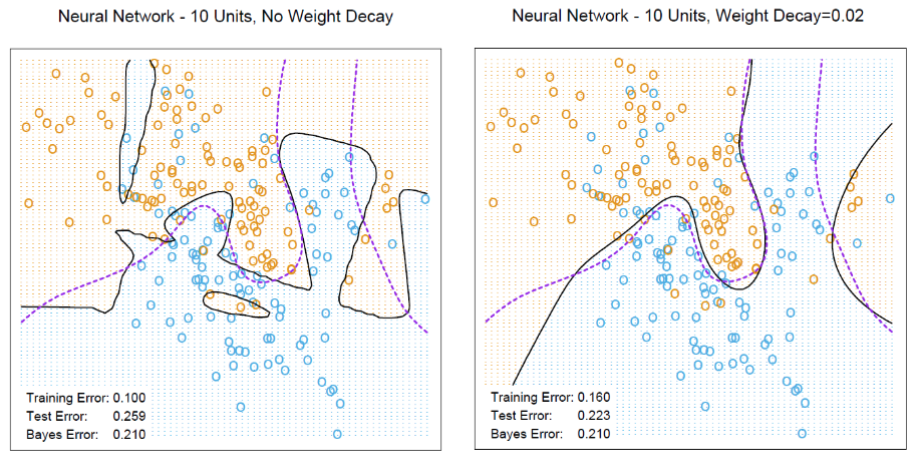
\includegraphics[width=0.8\textwidth]{fotos/45.png}
\caption{Resultado del entrenamiento de una red neuronal con diez unidades ocultas, sin decaimiento de peso (panel izquierdo) y con decaimiento de peso (panel derecho). El decaimiento de peso ha mejorado claramente la predicción.}
\label{fig:7.6}
\end{figure}

\subsection{Escalado de las entradas}

Dado que el escalado de las entradas determina el escalado efectivo de los pesos en la capa inferior, puede tener un gran efecto en la calidad de la solución final. Al principio, es mejor estandarizar todas las entradas para que tengan media cero y desviación estándar uno. Esto asegura que todas las entradas sean tratadas por igual en el proceso de regularización y permite elegir un rango significativo para los pesos iniciales aleatorios. Con entradas estandarizadas, es típico tomar pesos aleatorios uniformes en el rango $[-0.7, 0.7]$.

\subsection{Número de unidades ocultas y capas}

En general, es mejor tener demasiadas unidades ocultas que muy pocas. Con muy pocas unidades ocultas, el modelo podría no tener suficiente flexibilidad para capturar las no linealidades en los datos; con demasiadas unidades ocultas, los pesos adicionales pueden reducirse hacia cero si se utiliza una regularización adecuada. Típicamente, el número de unidades ocultas está en el rango de 5 a 100 (por capa), aumentando con el número de entradas y el número de casos de entrenamiento. \\

Es más común asignar un número razonablemente grande de unidades y entrenarlas con regularización. Algunos investigadores utilizan la validación cruzada para estimar el número óptimo, pero esto parece innecesario si se usa la validación cruzada para estimar el parámetro de regularización. \\

La elección del número de capas ocultas está guiada por el conocimiento previo y la experimentación. Cada capa extrae características de la entrada para regresión o clasificación. El uso de múltiples capas ocultas permite la construcción de características jerárquicas en diferentes niveles de resolución. Un ejemplo del uso efectivo de múltiples capas se dará más adelante.

\subsection{Múltiples mínimos}

La función de error no es convexa y posee muchos mínimos locales. Como resultado, la solución final obtenida depende bastante de la elección de los pesos iniciales. Es necesario al menos probar varias configuraciones iniciales aleatorias y elegir la solución que dé el error (penalizado) más bajo. \\

Un mejor enfoque es usar las predicciones promedio sobre la colección de redes como la predicción final. Esto es preferible a promediar los pesos, ya que la no linealidad del modelo implica que esta solución promediada podría ser bastante deficiente. Otro enfoque es a través del \textit{bagging}, que promedia las predicciones de redes entrenadas a partir de versiones perturbadas aleatoriamente del conjunto de entrenamiento. \\

Además, existen problemas con el descenso de gradiente: la pérdida cambia rápidamente en una dirección y lentamente en otra, la existencia de mínimos locales y puntos de silla (común en altas dimensiones) o el ruido en los gradientes generado por los mini lotes complican la búsqueda. Para solucionar estos inconvenientes, existen algoritmos de optimización más avanzados.

\subsection{Velocidad de aprendizaje}

Ya vimos que una velocidad de aprendizaje muy alta (mucho cambio en el peso $W$), nos aleja del mínimo en vez de acercarnos a él. Por ello, hay distintas estrategias para fijar el valor de la velocidad de aprendizaje:
\begin{itemize}
\item Tasa de aprendizaje fija: es la estrategia normal, muy usada en problemas reales.
\item Decaimiento de la tasa de aprendizaje cada cierto numero de iteraciones: los incrementos o decrementos se suelen hacer en factores de 10. 
\item Decaimiento exponencial: la tasa de aprendizaje se reduce exponencialmente con el número de iteraciones.
\begin{equation}
\alpha = \alpha_0 e^{-kt}
\end{equation} 
\item Decaimiento de la tasa de aprendizaje por 1/t: la tasa de aprendizaje se reduce por un factor de 1/t, donde t es el número de iteraciones.
\begin{equation}
\alpha = \frac{\alpha_0}{1 + kt}
\end{equation}
\item En la realidad, se suelee dejar sobreaprender a un modelo con una tasa fija. Luego, se recupera el modelo en un punto anterior al sobreajuste y se lanza un entrenamiento con una velocidad menor. Esto se repite una o dos veces. 
\begin{figure}[H]
\centering
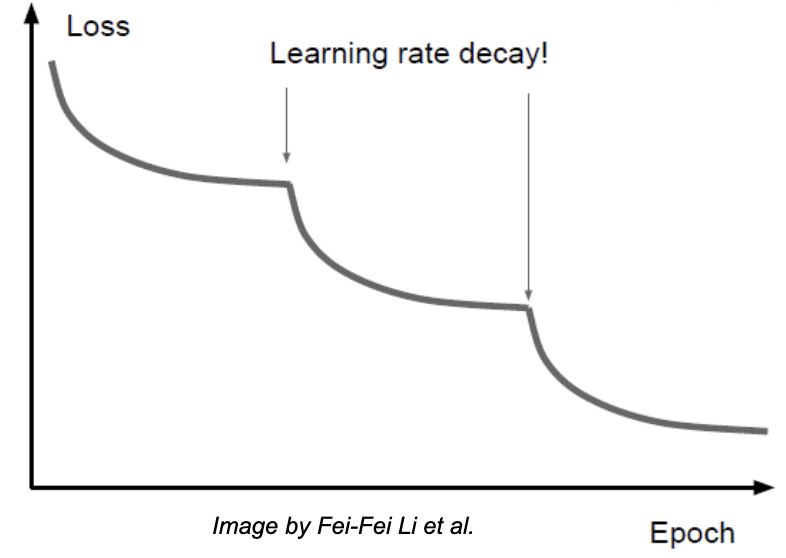
\includegraphics[width=0.6\textwidth]{fotos/49.png}
\end{figure}
\end{itemize}

\subsection{Hiperparámetros}

No se puede hacer exploracion exhaustiva de todos los valores de los hiperparámetros de una red neuronal. Primero se hace una búsqueda de grano grueso con pocas épocas y luego una de grano fino (aunque no exhaustiva) con un número mayor de épocas. Es muy importante ver la curva de aprendizaje para ver si el modelo esta sobre o subaprendiendo.

\subsection{Optimización}

\noindent El descenso de gradiente estocástico ``vanilla'' es el método más común para entrenar redes neuronales: 
\begin{equation}
W_{t+1} = W_t - \alpha \nabla J (W_t)
\end{equation}

Sin embargo, existen otros métodos más avanzados que pueden ser más rápidos y más efectivos. Algunos de estos métodos son:
\begin{itemize}
    \item Descenso de gradiente estocástico con momento: añadimos un componente de ``memoria'' que tiene en cuenta la velocidad previa. Esto permite sortear mínimos locales.
    \begin{equation}
        W_{t + 1} = W_t + v_{t + 1}, \quad v_{t + 1} = \rho v_t - \alpha \nabla J (W_t) 
    \end{equation}
    \begin{figure}[H]
    \centering
    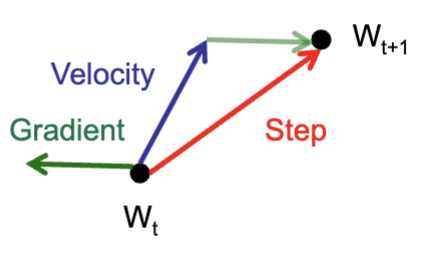
\includegraphics[width=0.3\textwidth]{fotos/50.png}
    \end{figure}
    \item Descenso de gradiente estocástico con momento de Nesterov: el gradiente se calcula en otro punto (el más actual) $W + \rho v_t$.
    \begin{equation}
        W_{t + 1} = W_t + v_{t + 1}, \quad v_{t + 1} = \rho v_t - \alpha \nabla J (W_t + \rho v_t)
    \end{equation}
    \begin{figure}[H]
    \centering
    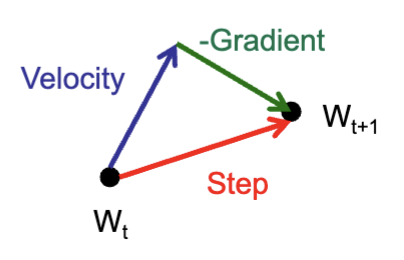
\includegraphics[width=0.3\textwidth]{fotos/51.png}
    \end{figure}
\end{itemize}

Hay otros algoritmos como AdaGrad, RMSProp, Adam, etc. que simplemente hacen correcciones de distintas formas al gradiente y a la velocidad de aprendizaje, de distintas formas. \\

Todos los metodos anteriores usan optimización de primer orden (basada en el gradiente). Sin embargo, hay métodos de segundo orden que usan la matriz hessiana como aproximación cuadrática. Esta matriz nos da informacion relativa al paso (al hacer una optimizacion de segundo orden se puede ignorar la tasa de aprendizaje). Para ello, se usa el metodo de Newton: hacemos una expansión de $J(W_{t + 1})$ en serie de Taylor
\begin{equation}
J(W_{t + 1}) = J(W_t) + \nabla J(W_t) \cdot (W_{t + 1} - W_t) + \frac{1}{2} (W_{t + 1} - W_t)^2 \nabla^2 J (W_t)  + \dots
\end{equation}

Para resolver respecto al punto crítico, derivamos respecto al paso $(W_{t + 1} - W_t)$ y actualizamos el valor como
\begin{equation}
W_{t + 1} = W_t - (\nabla^2 J (W_t))^{-1} \nabla J (W_t)
\end{equation}

La inversa del hessiano será lo que sirva de velocidad de aprendizaje. Si esta matriz tiene dimension de $k \times k$, el coste computacional de invertirla sería $\mathcal{O}(k^3)$, por lo que no es viable en \textit{deep learning}. Sin embargo, hay métodos ``quasi-Newton'' que aproximan la inversa de la matriz hessiana. El más popular de ellos es el \textit{Limited memory} BFGS (L-BFGS). \\

\noindent Como resumen general, en \textit{deep learning}:
\begin{itemize}
\item Adam es una buena elección.
\item Descenso de gradiente estocástico con momento y con una velocidad de aprendizaje que decaiga (la más común es dejar sobreaprender una o dos veces, recuperar el modelo antes de que esté sobreaprendido y luego reducir la velocidad de aprendizaje) necesita mayor ajuste, pero puede ser mejor que Adam.
\item L-BFGS no funciona bien con mini lotes, pero es una buena elección para problemas pequeños donde se pueda usar el lote completo.
\end{itemize}



Reglas practicas (para deep learning sobre todo)


\section{Ejemplo: datos de \textit{ZIP code}}

Este ejemplo es una tarea de reconocimiento de caracteres: clasificación de números manuscritos. La figura \ref{fig:7.7} muestra algunos ejemplos de dígitos escritos a mano normalizados, escaneados automáticamente desde sobres por el Servicio Postal de EE.UU. Estos 256 valores de píxeles se utilizan como entradas para el clasificador de red neuronal. \\

\begin{figure}[h]
\centering
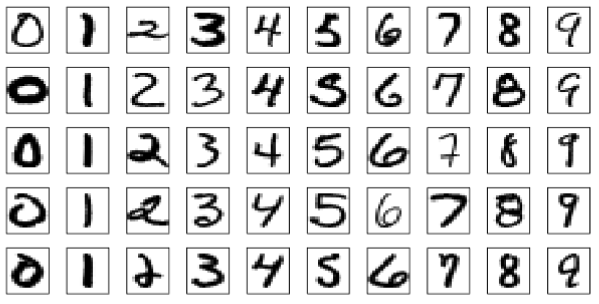
\includegraphics[width=0.8\textwidth]{fotos/46.png}
\caption{Ejemplos de dígitos escritos a mano normalizados. Los dígitos escaneados originales son binarios y de diferentes tamaños y orientaciones; las imágenes mostradas aquí han sido enderezadas y normalizadas en tamaño, resultando en imágenes en escala de grises de $16 \times 16$}
\label{fig:7.7}
\end{figure}

Una red neuronal de caja negra no es idealmente adecuada para esta tarea de reconocimiento de patrones, en parte porque la representación en píxeles de las imágenes carece de ciertas invariantes (como pequeñas rotaciones de la imagen). En consecuencia, los primeros intentos con redes neuronales arrojaron tasas de error de clasificación alrededor del $4.5$\% en varios ejemplos del problema. \\

Aunque los conjuntos de datos actuales de dígitos tienen decenas de miles de ejemplos de entrenamiento y prueba, el tamaño de la muestra aquí es deliberadamente modesto para enfatizar los efectos. Los ejemplos se obtuvieron escaneando algunos dígitos dibujados a mano reales y luego generando imágenes adicionales mediante desplazamientos horizontales aleatorios. Hay 320 dígitos en el conjunto de entrenamiento y 160 en el conjunto de prueba y se ajustaron cinco redes diferentes a los datos (figure \ref{fig:7.8}):
\begin{itemize}
\item Net-1: Sin capa oculta, equivalente a regresión logística multinomial.
\item Net-2: Una capa oculta, 12 unidades ocultas completamente conectadas.
\item Net-3: Dos capas ocultas con conexiones locales.
\item Net-4: Dos capas ocultas, conexiones locales con compartición de pesos.
\item Net-5: Dos capas ocultas, conexiones locales, dos niveles de compartición de pesos.
\end{itemize}

\begin{figure}[h]
\centering
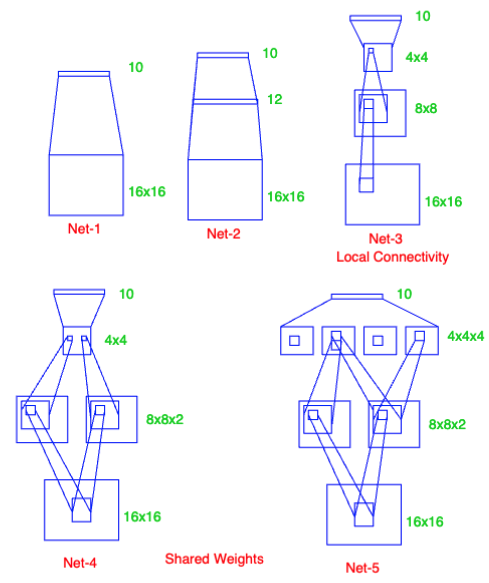
\includegraphics[width=0.8\textwidth]{fotos/47.png}
\caption{Arquitectura de las redes neuronales utilizadas en el ejemplo de reconocimiento de dígitos.}
\label{fig:7.8}
\end{figure}

Por ejemplo, Net-1 tiene 256 entradas, una para cada uno de los $16 \times 16$ píxeles de entrada, y diez unidades de salida para cada uno de los dígitos 0-9. El valor predicho $\hat{f}_k(x)$ representa la probabilidad estimada de que una imagen $x$ pertenezca a la clase de dígito $k$, para $k = 0, 1, 2, \dots, 9$. \\

Todas las redes tienen unidades de salida sigmoides y fueron todas entrenadas con la función de error de suma de cuadrados. La primera red no tiene capa oculta y, por lo tanto, es casi equivalente a un modelo de regresión multinomial lineal. Net-2 es una red de una sola capa oculta con 12 unidades ocultas, del tipo descrito anteriormente.

\begin{figure}[h]
\centering
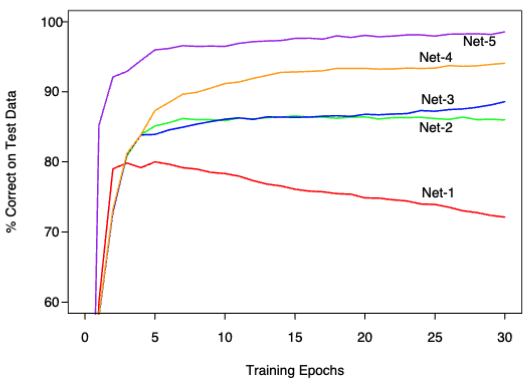
\includegraphics[width=0.8\textwidth]{fotos/48.png}
\caption{Curvas de rendimiento de \textit{test} como función del número de épocas de entrenamiento para las redes neuronales Net-1 a Net-5.}
\label{fig:7.9}
\end{figure}

El error en el conjunto de entrenamiento para todas las redes fue del 0\%, ya que en todos los casos hay más parámetros que observaciones de entrenamiento. La evolución del error de prueba durante las épocas de entrenamiento se muestra en la figura \ref{fig:7.9}. La red lineal (Net-1) comienza a sobreajustarse bastante rápido, mientras que el rendimiento en la prueba de las otras redes se estabiliza en valores sucesivamente superiores. \\

Las otras tres redes tienen características adicionales que demuestran el poder y la flexibilidad del paradigma de redes neuronales. Introducen restricciones en la red, naturales para el problema en cuestión, que permiten una conectividad más compleja pero con menos parámetros. \\

Net-3 utiliza conectividad local: esto significa que cada unidad oculta está conectada solo a un pequeño parche de unidades en la capa inferior. En la primera capa oculta (una matriz de $8 \times 8$), cada unidad toma entradas de un parche de $3 \times 3$ de la capa de entrada; para unidades en la primera capa oculta que están a una unidad de distancia, sus campos receptivos se superponen por una fila o columna, y por lo tanto están a dos píxeles de distancia. En la segunda capa oculta, las entradas provienen de un parche de $5 \times 5$, y nuevamente las unidades que están a una unidad de distancia tienen campos receptivos que están a dos unidades de distancia. Los pesos para todas las demás conexiones se establecen a cero. La conectividad local hace que cada unidad sea responsable de extraer características locales de la capa inferior y reduce considerablemente el número total de pesos. Con muchas más unidades ocultas que Net-2, Net-3 tiene menos enlaces y, por lo tanto, menos pesos, logrando un rendimiento similar. \\

Net-4 y Net-5 tienen conectividad local con \textbf{compartición de pesos}\footnote{Descenso de gradiente con comparticion de pesos: medimos el error para todas las neuronas controladas con el mismo peso y hacemos la media.}. Todas las unidades en un mapa de características local realizan la misma operación en diferentes partes de la imagen, lograda compartiendo el mismo conjunto de pesos. La primera capa oculta de Net-4 tiene dos matrices de $8 \times 8$, y cada unidad toma entrada de un parche de $3 \times 3$ al igual que en Net-3 Una de las dos capas $8 \times 8$ busca una característica, y la otra, otra característica. Sin embargo, cada una de las unidades en un único mapa de características de $8 \times 8$ comparte el mismo conjunto de nueve pesos (pero tienen su propio parámetro de sesgo). Esto fuerza a que las características extraídas en diferentes partes de la imagen sean computadas por la misma función lineal, y en consecuencia, estas redes a veces se conocen como redes convolucionales. La segunda capa oculta de Net-4 no tiene compartición de pesos y es la misma que en Net-3. El gradiente de la función de error respecto a un peso compartido es la suma de los gradientes de $J$ respecto a cada conexión controlada por los pesos en cuestión. \\

\begin{table}[h]
\centering
\begin{tabular}{ccccc}
\hline \hline 
 & Arquitectura & Enlaces & Pesos (aprendidos) & \% correctitud \\ \hline \hline 
Net-1 & Una única capa & 2570 & 2570 & 80.0 \\
Net-2 & Una capa oculta & 3214 & 3214 & 87.0 \\
Net-3 & Dos capas ocultas & 1226 & 1226 & 88.5 \\
Net-4 & Red restringida 1 & 2266 & 1132 & 94.0 \\
Net-5 & Red restringida 2 & 5194 & 1060 & 98.4 \\ \hline
\end{tabular}
\label{tab:7.1}
\end{table}

La conectividad local hace que se tengan que aprender menos peso. La tabla \ref{tab:7.1} da el número de enlaces, el número de pesos y el rendimiento óptimo en la prueba para cada una de las redes. Vemos que Net-4 tiene más enlaces pero menos pesos que Net-3, y un rendimiento en prueba superior. Net-5 tiene cuatro mapas de características de $4 \times 4$ en la segunda capa oculta, cada unidad conectada a un parche local de $5 \times 5$ en la capa inferior. Los pesos se comparten en cada uno de estos mapas de características. Vemos que Net-5 es la mejor, con errores de solo 1.6\%, comparado con el 13\% para la red \textit{vanilla} Net-2. El diseño ingenioso de la red Net-5, motivado por el hecho de que las características del estilo de escritura a mano deberían aparecer en más de una parte de un dígito, fue el resultado de muchos años de experimentación. Esta y redes similares dieron un mejor rendimiento en problemas de códigos ZIP que cualquier otro método de aprendizaje en ese momento (principios de los años 1990). Este ejemplo también muestra que las redes neuronales no son una herramienta completamente automática, como a veces se anuncian. Como con todos los modelos estadísticos, el conocimiento del tema puede y debe utilizarse para mejorar su rendimiento. \\

Esta red fue posteriormente superada por el enfoque de distancia tangente, que incorpora explícitamente invariantes afines naturales. En este punto, los conjuntos de datos de reconocimiento de dígitos se convierten en bancos de pruebas para cada nuevo procedimiento de aprendizaje, y los investigadores trabajaron arduamente para reducir las tasas de error. Por ahora, las mejores tasas de error en una base de datos grande (60000 de entrenamiento, 10000 de prueba), derivadas de bases de datos estándar NIST\textsuperscript{2}, se reportaron de la siguiente manera:
\begin{itemize}
\item 1.1\% para distancia tangente con un clasificador de vecino más cercano.
\item 0.8\% para una SVM polinomial de grado 9.
\item 0.8\% para LeNet-5, una versión más compleja de la red convolucional descrita aquí.
\item 0.7\% para LeNet-4 potenciado. LeNet-4 es un predecesor de LeNet-5.
\end{itemize}



